\documentclass[12pt]{article}
\usepackage{array,tabularx}
\usepackage{graphicx}
\usepackage{float}
\usepackage{amsmath}
\setlength{\parindent}{0pt}

\newenvironment{conditions}
	{\par\vspace{\abovedisplayskip}\noindent
	\tabularx{\columnwidth}{>{$}l<{$}@{}>{${}}c<{{}$}@{} >{\raggedright\arraybackslash}X}}
	{\endtabularx\par\vspace{\belowdisplayskip}}

\title{Reaction Kinetics Lab Report}
\author{Ben Hammond}
\date{\today}


\begin{document}
	\maketitle
	\newpage

	\section{Purpose}
	The purpose of this lab was to experimentally determine the reaction kinetics for the decomposition of hydrogen peroxide ($\text{H}_2\text{O}_2$) with a catalyst of potassium iodide (KI), including the reaction rate and activation energy.
	
	\section{Procedure}
	A glass cup was first filled with water up to the brim. A 100 m: graduated cylinder was then filled completely with water, and was then inverted into the cup such that no air entered the graduated cylinder. Two glasses of the same height as the first were placed on either side of the water filled one, and two wine glasses were placed on top of the glasses, each one balanced between the water filled glass and one of the two other glasses. The graduated cylinder was then lifted upward and balanced upon the rims of the wine glasses. A long rubber tube with one end inserted into a stopper for a test tube was fed into the water filled graduated cylinder such that the end of tube opposite of the stopper was placed approximately halfway up inside of the graduated cylinder. 6 mL of approximately 3\% $\text{H}_2\text{O}_2$ was measured in a separate graduated cylinder and poured into a test tube. 15 drops of KI were then added to the test tube, and the end of the rubber tubing with the stopper was quickly used to seal the test tube. The volume of $\text{O}_2$ gas collected in the graduated cylinder was measured every thirty seconds until the reaction slowed to an unnoticeable rate.
	
	The setup was then disassembled, cleaned, and reassembled. The second version of the experiment involved holding the reaction at a constant temperature of 50$^\circ$C, which required slight modifications to the experimental setup. The existing setup was moved next to a gas stove top, on top of which was placed a large, flat, metal griddle. This was heated on one end by a low flame until hot. In the middle of the griddle was placed a large metal pot of ice water. At the far end of the griddle, farthest away from the flame, was placed a small pot of water into which the reaction test tube was placed. This allowed the reaction to be kept at a semi-stable temperature, which was kept close to 50$^\circ$C by periodically adding cold water to decrease the temperature or moving it closer to the heat source to increase the temperature. In this way a temperature close to 50$^\circ$C (varying only by a degree or so) was maintained throughout the duration of the reaction. As before, the reaction was started, and the $\text{O}_2$ output was measured throughout the reaction.

	\begin{figure}[H]
		\centerline{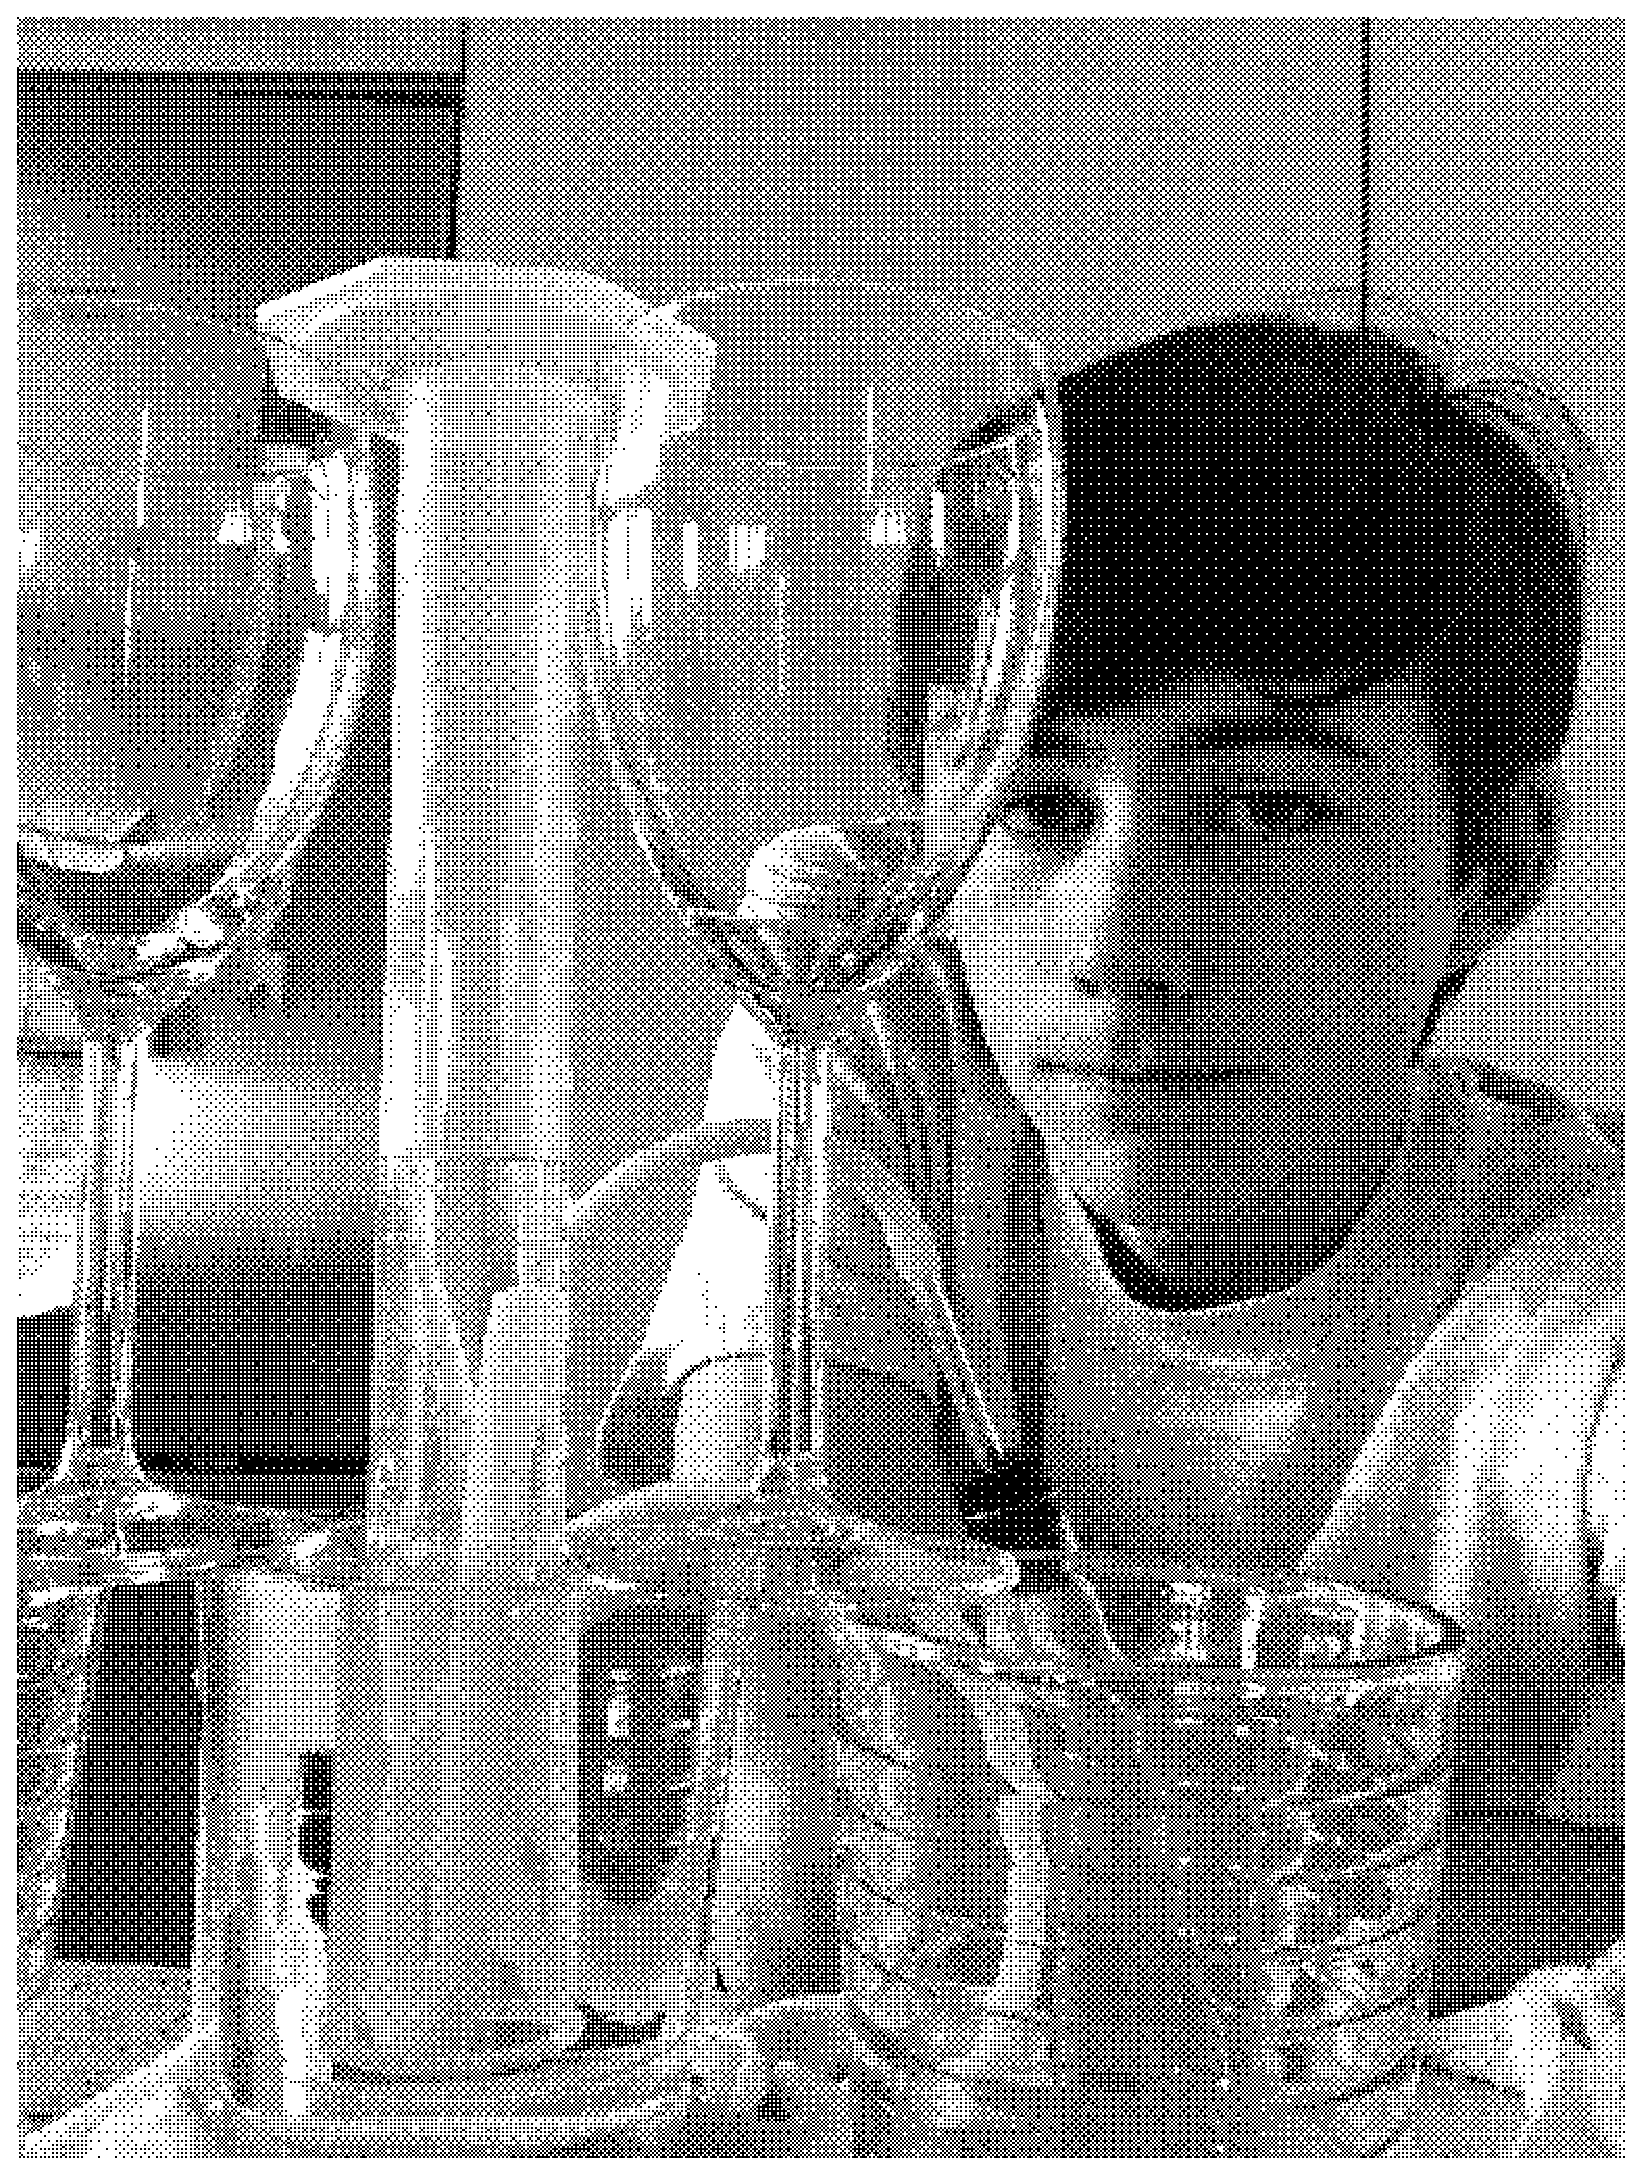
\includegraphics[width=.5\textwidth]{images/selfie.EPS}}
		\caption{A photo of myself with the experimental setup}
	\end{figure}

	\section{Data}
	\begin{flushleft}
	\begin{tabular}{ l|l|l }
		time (s) & V at 22.5$^\circ$C (mL) & V at 50$^\circ$C (mL) \\
		\hline
		30 & 5 & 19 \\
		60 & 8 & 36 \\
		90 & 13 & 48 \\
		120 & 19 & 53 \\
		150 & 24 & 55 \\
		180 & 29 & 57 \\
		210 & 33 & 58 \\
		240 & 37 & 58.2 \\
		270 & 40 & 58.5 \\
		300 & 42 & 59 \\
		330 & 45 & 59.1 \\
		360 & 47 & 59.2 \\
		390 & 49 & 59.3 \\
		420 & 50 & 59.4 \\
		450 & 51 & 59.5 \\
		480 & 52 & 59.9 \\
		510 & 53 & 60 \\
		540 & 53.5 & 60 \\
		570 & 54 & 60.1 \\
		600 & 54.5 & 60.1 \\
		630 & 55 & 60.2 \\
		660 & 55.5 & 60.2 \\
		690 & 56 & 60.3 \\
		720 & 56.1 & 60.5 \\
		750 & 56.3 & 60.6 \\
		780 & 56.5 & 60.8 \\
		810 & 56.9 & 60.9 \\
		840 & 57 & 60.9 \\
		870 & 57.1 & 61 \\
		900 & 57.25 & 61 \\
		930 & 57.5 & 61 \\
		960 & 57.6 & 61 \\
		990 & 57.8 & 61.1
	\end{tabular}
	\end{flushleft}

	\section{Analysis}
	With these data, the concentrations of H$_2$O$_2$ were calculated using the following formula
	\begin{equation}
	\label{concentration}
		[\text{H}_2\text{O}_2] = M_0 - \frac{2 * V_{O_2} * 0.977\text{ atm}}{R * T * 0.0060\text{ L}}
	\end{equation}
	where
	\begin{conditions}
		M_0 & = & initial molarity \\
		V_{O_2} & = & volume of oxygen \\
		R & = & gas constant \\
		T & = & temperature in Kelvin
	\end{conditions}
	The initial molarity was calculated by using the above equation, but setting the final concentration to 0 and solving for initial concentration given temperature and final volume. For the reaction at 22.5$^\circ$C, this was solved as follows:
	$$ 0\text{ M} = M_0 - \frac{2*0.0578\text{ L}*0.977\text{ atm}}{0.08206\text{ L}\cdot\text{atm}/\text{K}\cdot\text{mol}*295.5\text{ K}*0.0060\text{ L}} $$
	$$ M_0 = \frac{0.11294\text{ L}\cdot\text{atm}}{0.14549\text{ L}^2\cdot\text{atm}/\text{mol}} $$
	$$ M_0 = 0.779\text{ M} $$
	The initial molarity for the reaction at 50$^\circ$C was solved for using the same method:
	$$ 0\text{ M} = M_0 - \frac{2*0.061\text{ L}*0.977\text{ atm}}{0.08206\text{ L}\cdot\text{atm}/\text{K}\cdot\text{mol}*323\text{ K}*0.0060\text{ L}} $$
	$$ M_0 = \frac{0.11939\text{ L}\cdot\text{atm}}{0.1590\text{ L}^2\cdot\text{atm}/\text{mol}} $$
	$$ M_0 = 0.751\text{ M} $$
	Using these initial concentrations and equation \ref{concentration}, data tables for concentration as a function of time were found
	\begin{flushleft}
	\begin{tabular}{ l|l|l }
		time (s) & M at 22.5$^\circ$C (M) & M at 50$^\circ$C (M) \\
		\hline
		0 & 0.7790 & 0.7510 \\
		30 & 0.7118 & 0.5176 \\
		60 & 0.6716 & 0.3087 \\
		90 & 0.6044 & 0.1612 \\
		120 & 0.5238 & 0.09980 \\
		150 & 0.4567 & 0.07523 \\
		180 & 0.3895 & 0.05065 \\
		210 & 0.3358 & 0.03836 \\
		240 & 0.2821 & 0.03591 \\
		270 & 0.2418 & 0.03222 \\
		300 & 0.2149 & 0.02608 \\
		330 & 0.1746 & 0.02485 \\
		360 & 0.1478 & 0.02362 \\
		390 & 0.1209 & 0.02239 \\
		420 & 0.1075 & 0.02116 \\
		450 & 0.09406 & 0.01993 \\
		480 & 0.08063 & 0.01871 \\
		510 & 0.06720 & 0.01502 \\
		540 & 0.06048 & 0.01379 \\
		570 & 0.05377 & 0.01379 \\
		600 & 0.04705 & 0.01256 \\
		630 & 0.04034 & 0.01256 \\
		660 & 0.03362 & 0.01133 \\
		690 & 0.02691 & 0.01133 \\
		720 & 0.02556 & 0.01011 \\
		750 & 0.02288 & 0.007648 \\
		780 & 0.02019 & 0.006419 \\
		810 & 0.01482 & 0.003962 \\
		840 & 0.01348 & 0.002733 \\
		870 & 0.01213 & 0.002733 \\
		900 & 0.01012 & 0.001504 \\
		930 & 0.006760 & 0.001504 \\
		960 & 0.005417 & 0.001504 \\
		990 & 0.002731 & 0.001504
	\end{tabular}
	\end{flushleft}
	By graphing functions of $\ln{\text{concentration}}$ for the reactions at 22.5$^\circ$C and 50$^\circ$C and then applying lines of best fit, reaction rates were found to be $5.21 \times 10^{-3}$ at 22.5$^\circ$C and $5.32 \times 10^{-3}$ at 50$^\circ$C:
	\begin{figure}[H]
		\centerline{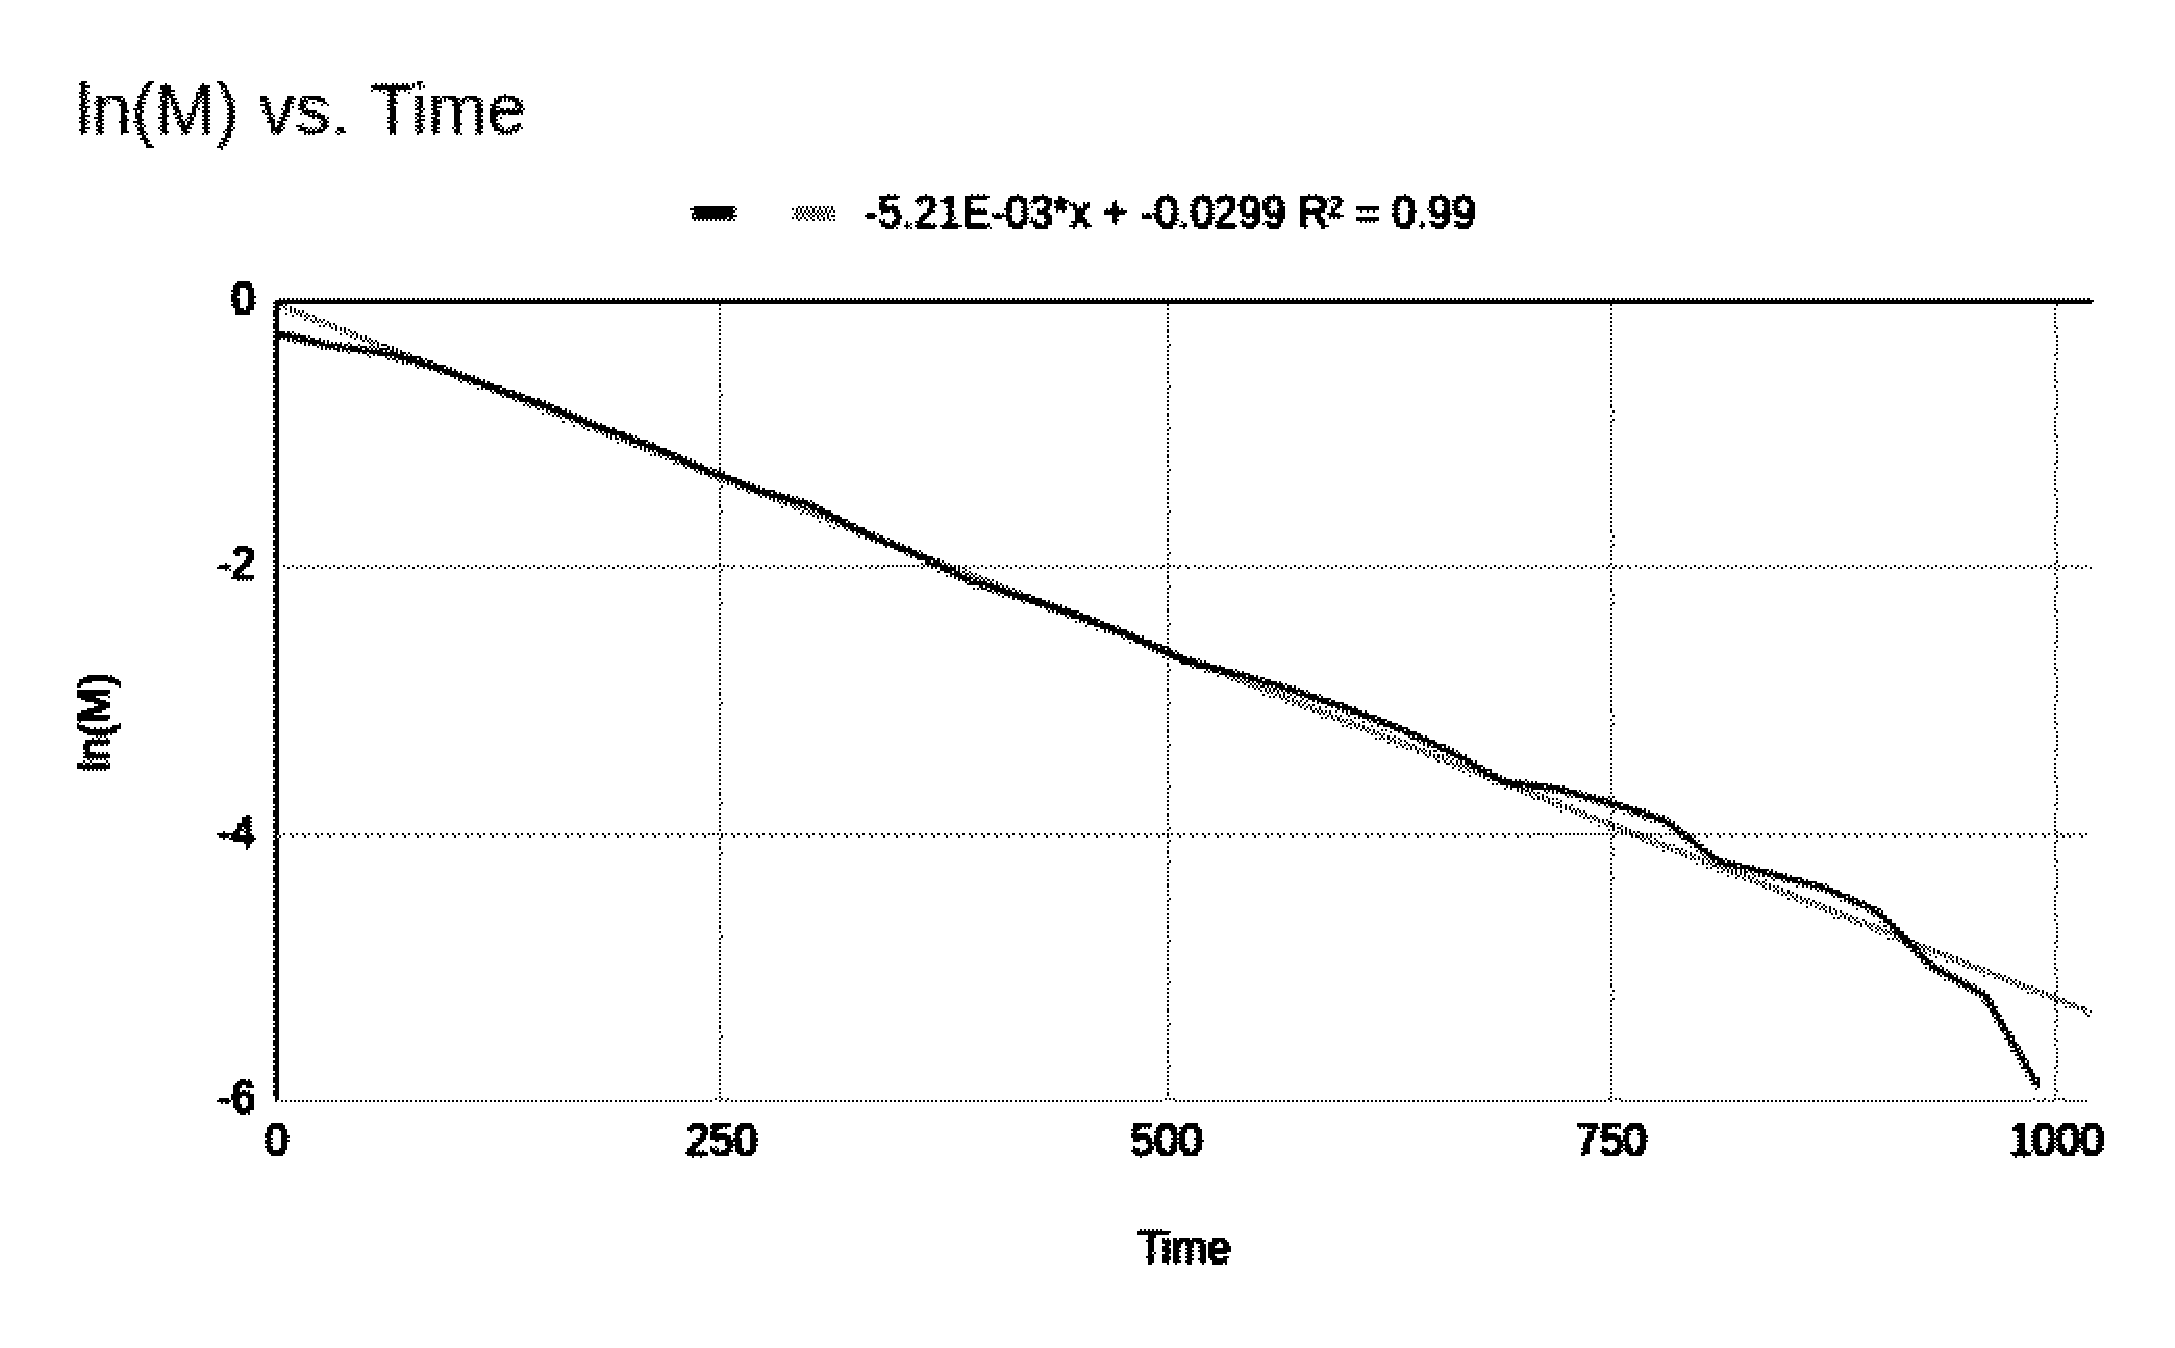
\includegraphics[width=.5\textwidth]{images/lnMvstime225.EPS}}
		\caption{A graph of the natural log of concentration as a function of time at 22.5$^\circ$C, with a line of best fit}
	\end{figure}
	\begin{figure}[H]
		\centerline{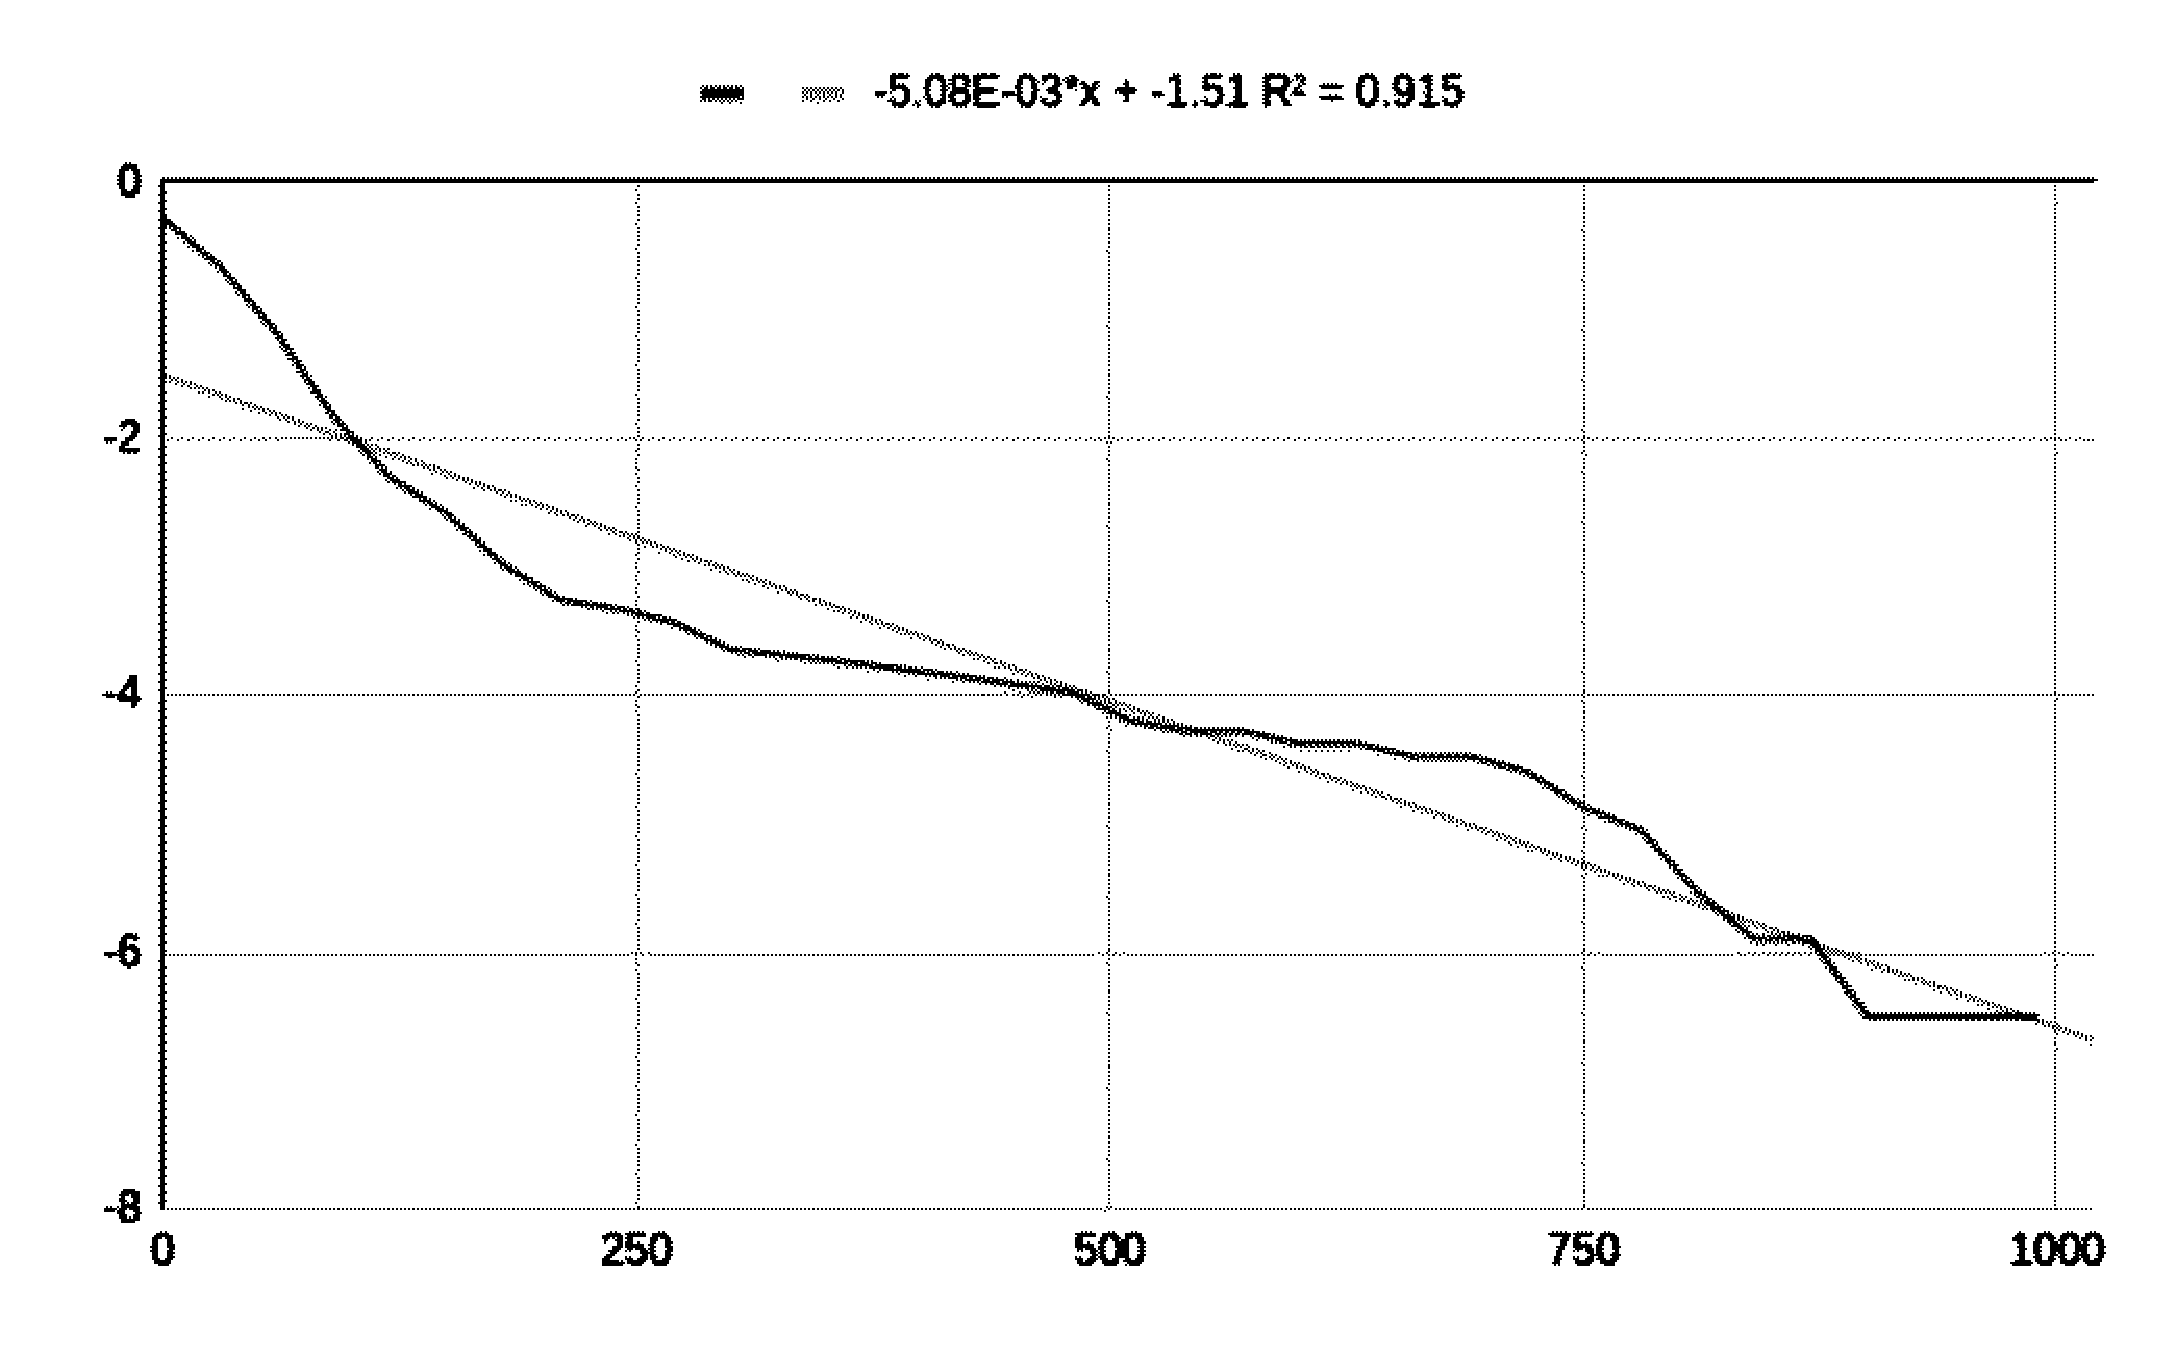
\includegraphics[width=0.5\textwidth]{images/lnmvstime50.EPS}}
		\caption{A graph of the natural log of concentration as a function of time at 50$^\circ$C, with a line of best fit}
	\end{figure}
	
	The natural log of reaction rates for temperatures between 5$^\circ$C and 50$^\circ$C, in increments of 5$^\circ$C, were plotted as a function of one over time, and a line of best fit was applied:
	\begin{figure}[H]
		\centerline{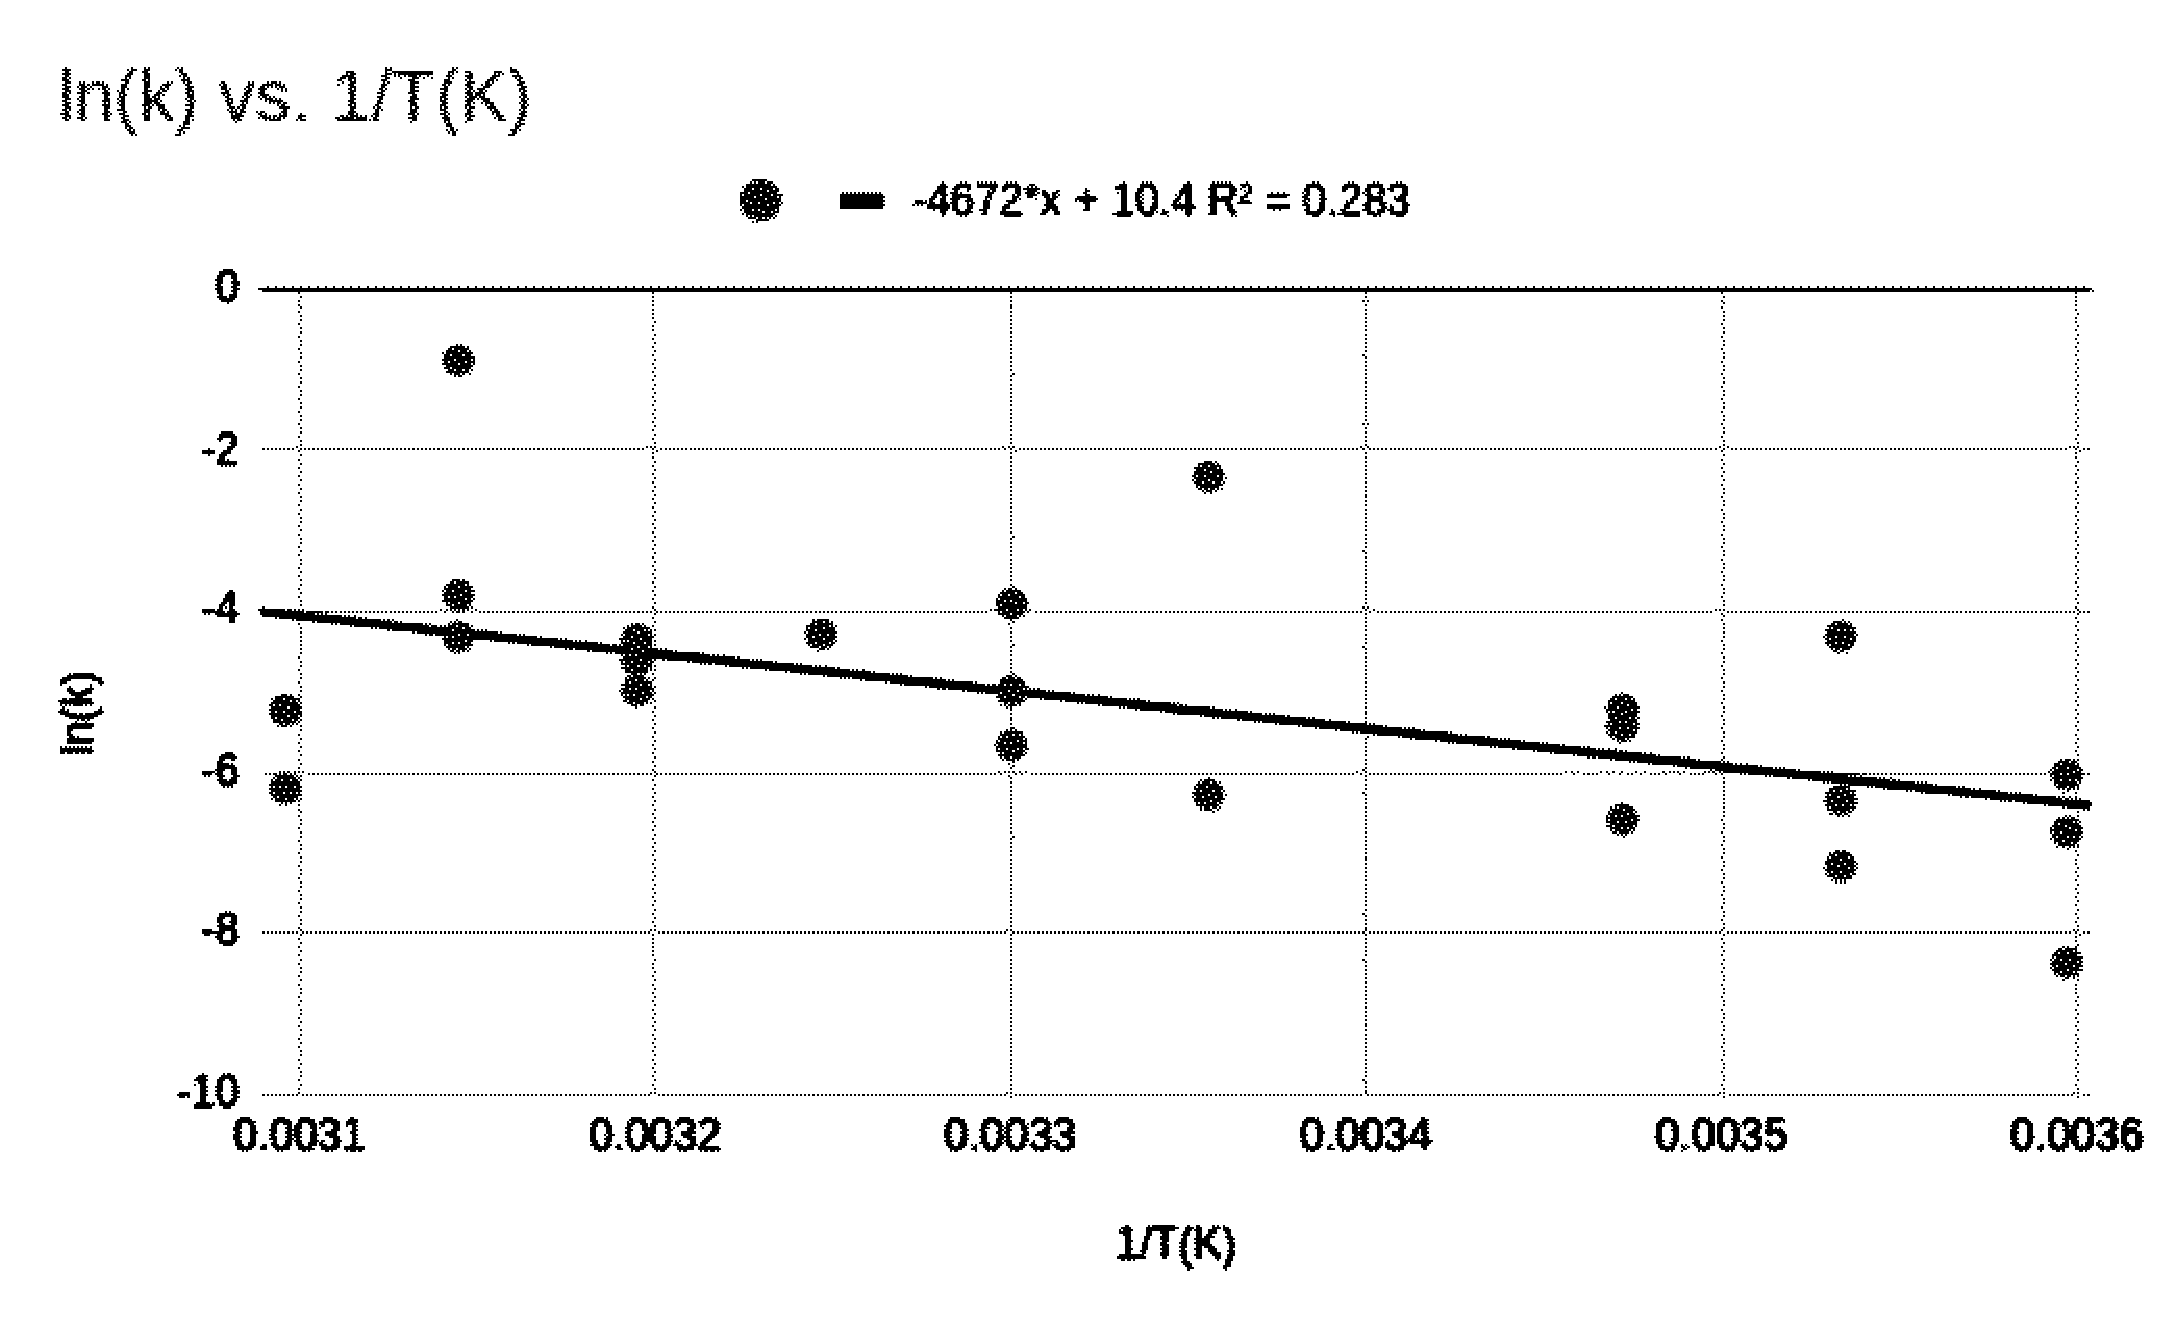
\includegraphics[width=0.5\textwidth]{images/initial_scatter.EPS}}
		\caption{A data plot of ln(k) as a function of 1/T}
	\end{figure}
	The raw data was significantly scattered though, with an initial R$^2$ value of 0.283. The initial data set was reduced by four data points which seemed likely as outliers, and the line of best fit was recalculated, with an R$^2$ value of 0.584:
	\begin{figure}[H]
		\centerline{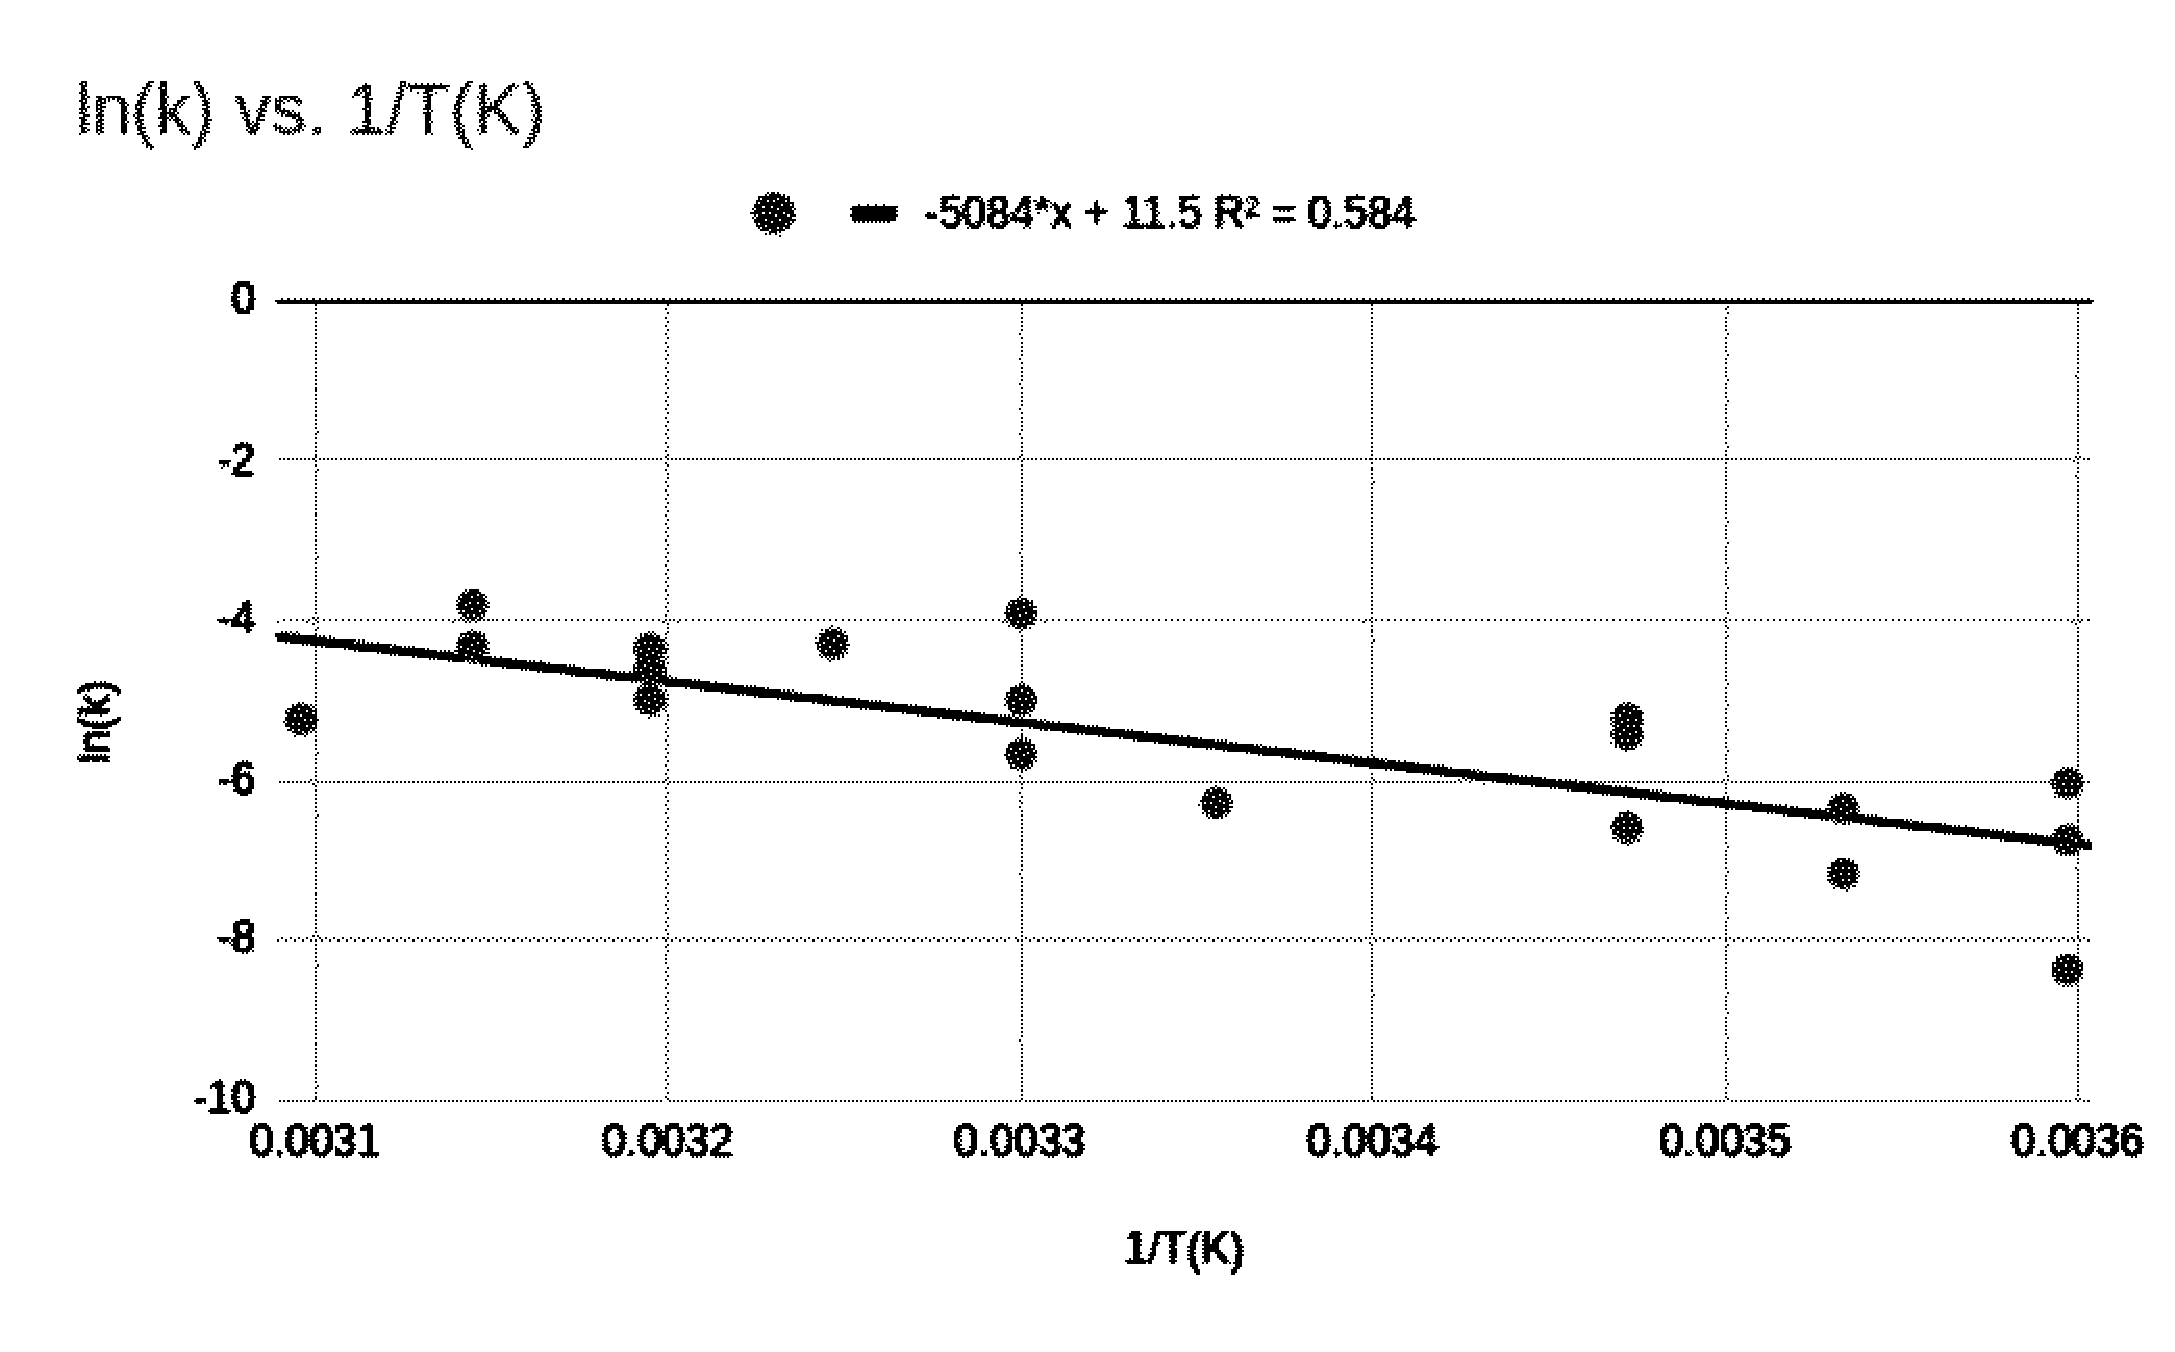
\includegraphics[width=0.5\textwidth]{images/second_scatter.EPS}}
		\caption{A modified data plot of ln(k) as a function of 1/T, with the outliers removed}
	\end{figure}
	By using the slope of this line, -5084, and the Arrhenius equation:
	\begin{equation}
	\label{arrhenius}
		\ln{k} = \frac{-E_a}{R}\cdot\frac{1}{T} + \ln{A}
	\end{equation}
	where
	\begin{conditions}
		k & = & reaction rate \\ 
		E_a & = & activation energy \\
		R & = & gas constant (8.32 J/K) \\
		T & = & temperature in Kelvin
	\end{conditions}
	the activation energy was found by solving:
	$$ -5084\text{ K} = \frac{-E_a}{R} $$
	$$ -5084\text{ K} = \frac{-E_a}{8.32\text{ J}\cdot\text{K}^{-1}\cdot\text{mol}^{-1}} $$
	$$ -42299\text{ J/mol} = -E_a $$
	$$ E_a = 42299\text{ J/mol} $$
	
	\section{Conclusions}
	The lab notebook pages in which this experiment was recorded are as follows:
	\begin{figure}[H]
	  \centering
	  \begin{minipage}[b]{0.4\textwidth}
	    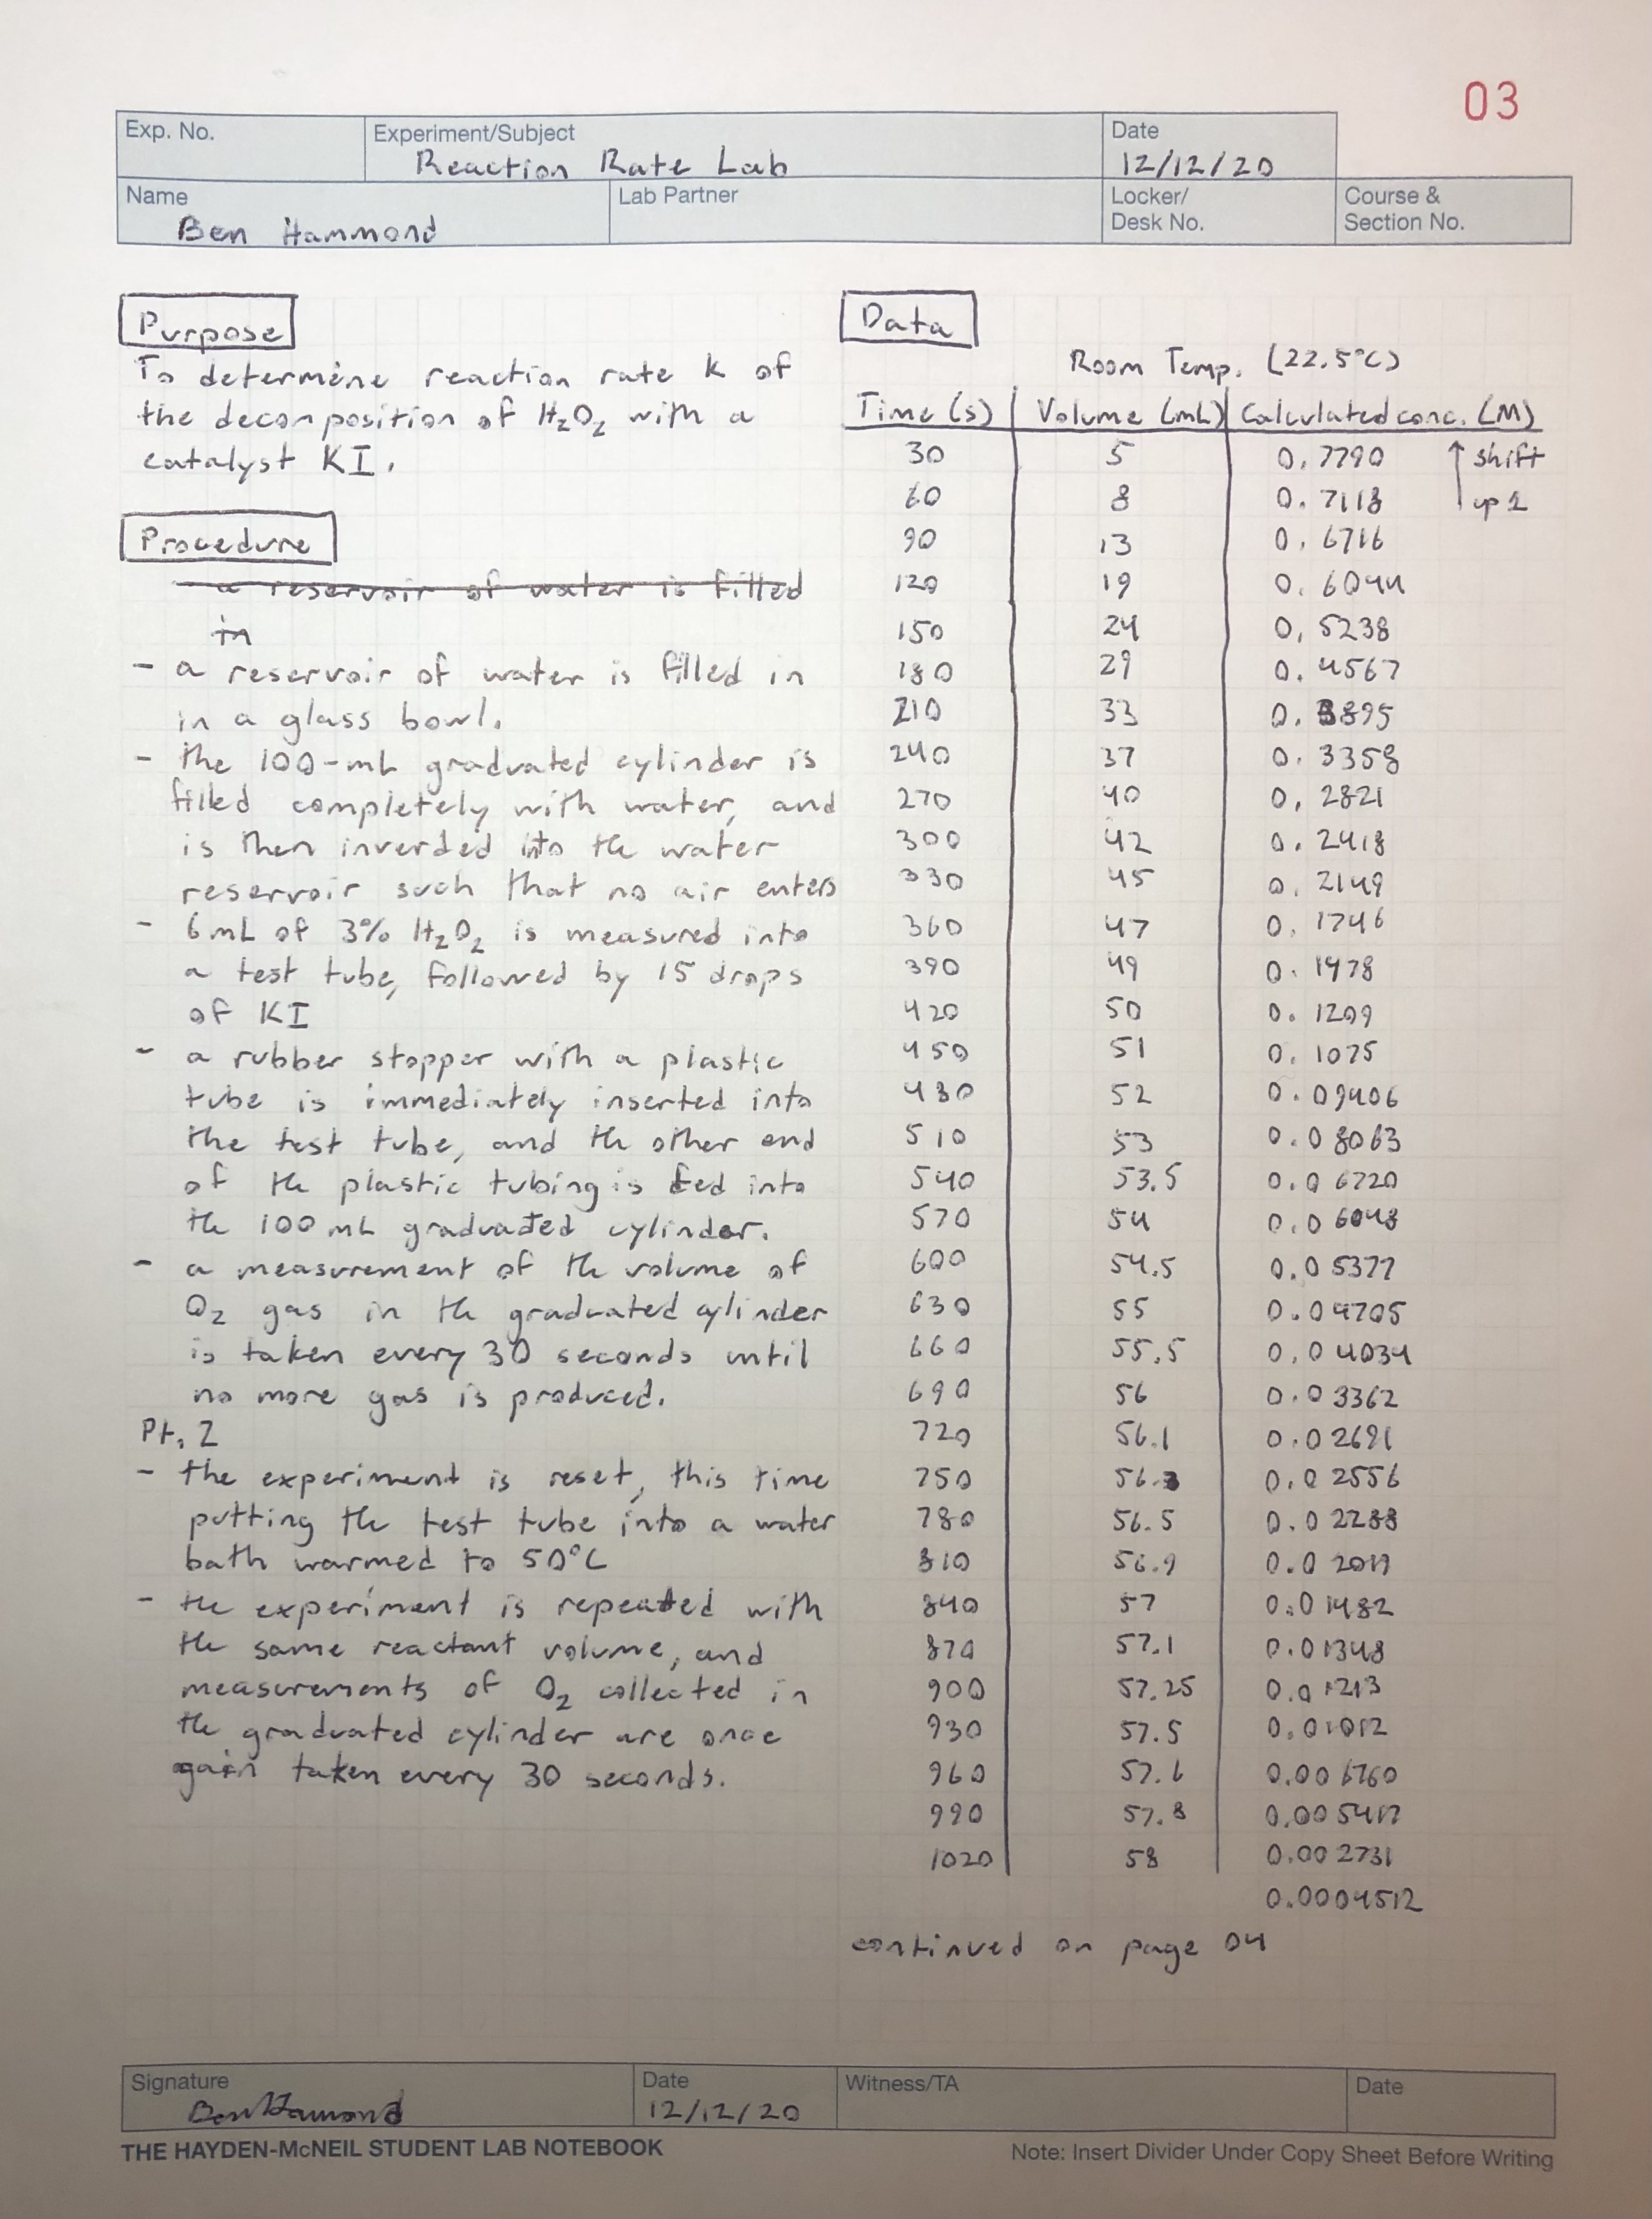
\includegraphics[width=\textwidth]{images/page1.EPS}
	    \caption{The first page of this experiment in a lab notebook.}
	  \end{minipage}
	  \hfill
	  \begin{minipage}[b]{0.4\textwidth}
	    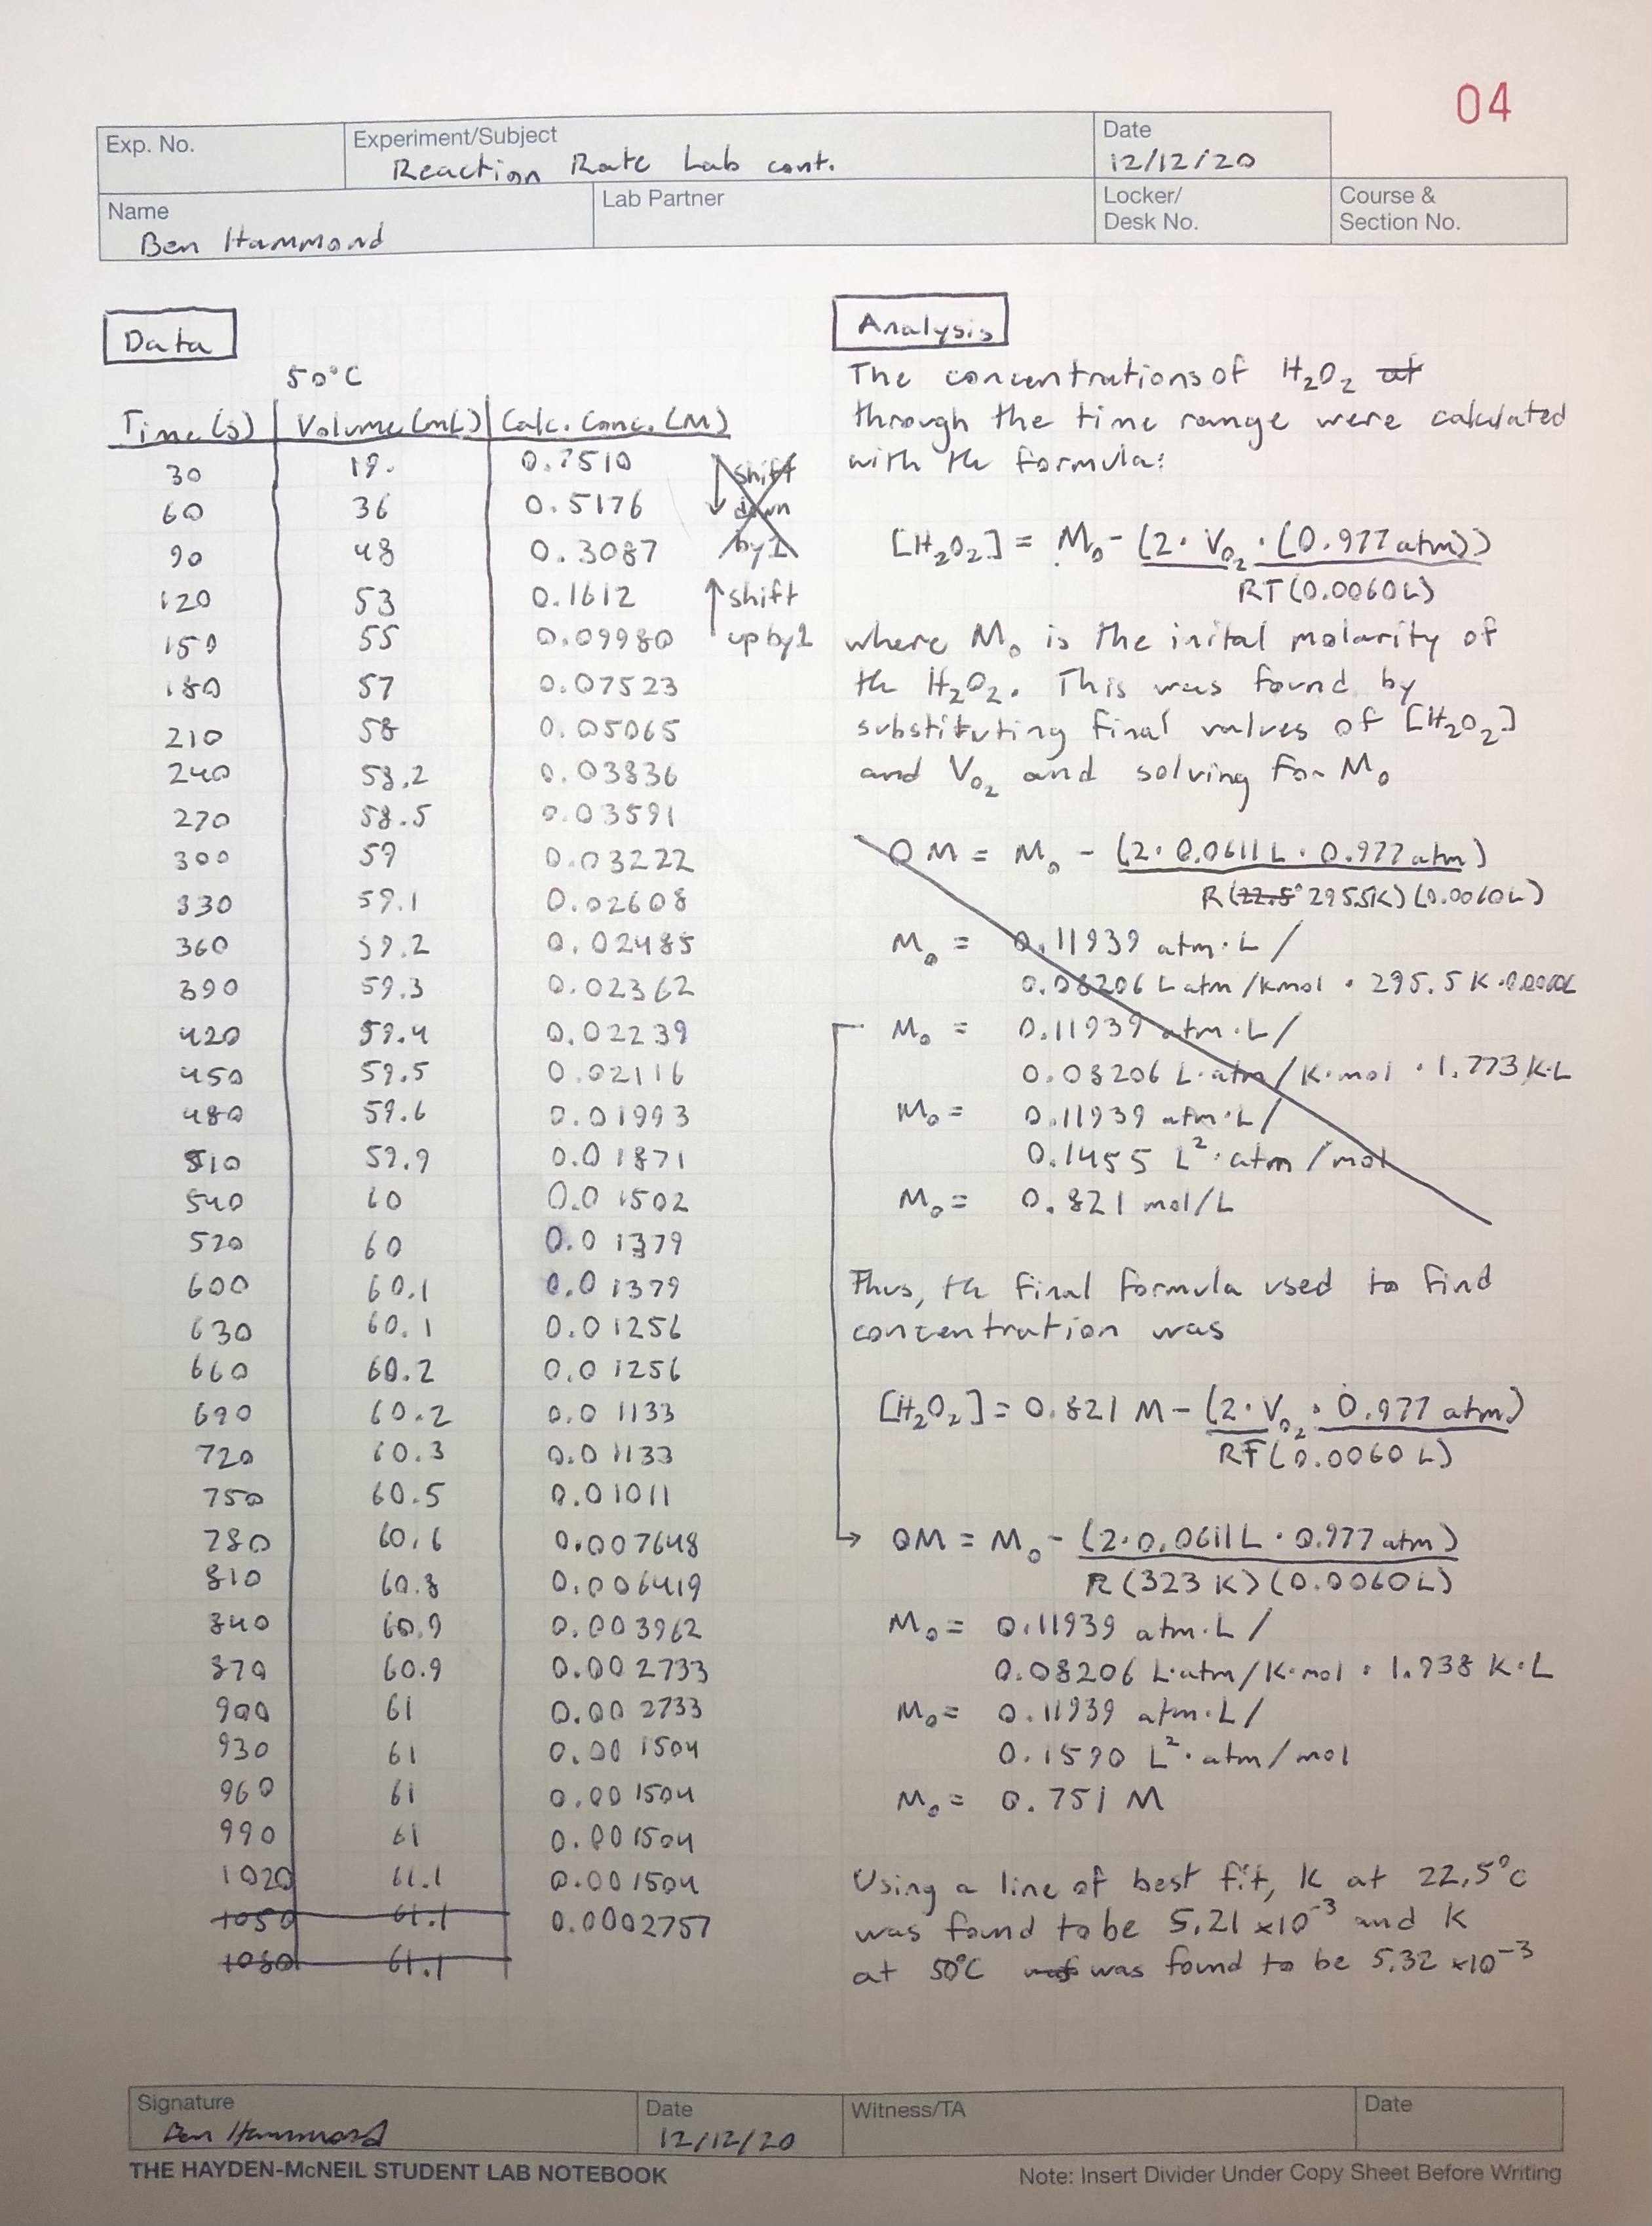
\includegraphics[width=\textwidth]{images/page2.EPS}
	    \caption{The second page of this experiment}
	  \end{minipage}
	\end{figure}
	These results are certainly far from the actual values. The experiments done to obtain the necessary data were done under deeply sub-optimal conditions, with little access to proper lab ware. As such, the results are likely very inaccurate. This point is further made by the wide spread of data in the table of reaction rates produced by the class. 
	
\end{document}
